\documentclass[letterpaper]{article}
\usepackage[submission]{aaai2027}
\usepackage[hyphens]{url}
\usepackage{graphicx}
\urlstyle{rm}
\def\UrlFont{\rm}
\usepackage{natbib}
\usepackage{caption}
\usepackage{booktabs}
\usepackage{array}
\usepackage{tabularx}
\usepackage{amsmath}
\usepackage{amssymb}
\frenchspacing

\pdfinfo{
/TemplateVersion (2027.1)
}

\setcounter{secnumdepth}{2}
\renewcommand{\thetable}{S\arabic{table}}
\renewcommand{\thefigure}{S\arabic{figure}}
\newcolumntype{L}[1]{>{\raggedright\arraybackslash}p{#1}}
\newcolumntype{Y}{>{\raggedright\arraybackslash}X}

\title{Supplementary Material for\\
The Cap Moves Answer Geometry, Not the Reasoning Trace: Representational--Policy Decoupling under Assistant-Axis Capping}
\author{Anonymous Submission}
\affiliations{}

\begin{document}
\maketitle

This supplement documents the data-construction pipeline, frozen experimental contracts, complete estimates, integrity checks, and the sequence of hypothesis tests behind the main paper.  Evidence and Social are separate audit modules with different source populations and resampling units; we never pool them into a single treatment effect.  All references to files below are stable identifiers inside the anonymous artifact archive, not public links.

\appendix

\section{Audit Scope and Outcome Contract}
\label{supp:contract}

\subsection{What is held fixed}

Every paired comparison fixes the base question, the model's initial answer $a_0$, the non-initial candidate $a_t$, option order, output contract, and all text outside the intended contrast.  CEDAR-Evidence changes the warrant attached to one proposed edit.  CEDAR-Social holds target exposure fixed and changes only social framing.  Table~\ref{tab:supp-contract} states the normative action and the estimand supported by each arm.

\begin{table*}[t]
\centering
\small
\begin{tabular}{llclL{3.2cm}L{4.6cm}}
\toprule
Module & Arm & $a_t$ shown & New support & Normative action & Primary diagnostic role \\
\midrule
Evidence & $N$ & No & None & Retain $a_0$ & Target-hidden neutral continuation; detects broad movement without a proposal. \\
Evidence & $R$ & No & None & Retain $a_0$ & Target-hidden request to recheck; separates reconsideration from evidence. \\
Evidence & $V$ & Yes & Sufficient & Update to $a_t$ & Warranted revision under a solver-certified valid argument. \\
Evidence & $F$ & Yes & Insufficient & Retain $a_0$ & Unwarranted revision under a single certified fatal inference. \\
Social & $AO$ & Yes & None & Retain $a_0$ & Pure target exposure without a speaker, evidence, authority, reward, or consensus. \\
Social & $S$ & Yes & None & Retain $a_0$ & $AO$ plus first-person confidence and a request to reconsider. \\
\bottomrule
\end{tabular}
\caption{\textbf{Paired audit contract.} ``Shown'' indicates whether $a_t$ appears in the follow-up.  Conditions are paired only within a module.}
\label{tab:supp-contract}
\end{table*}

\subsection{Discrete outcomes and continuous geometry}

Every generated answer is classified as \emph{initial}, \emph{induced target}, \emph{other wrong}, or \emph{invalid/abstain}.  This four-way coding prevents a reduction in target following from being misreported as an accuracy gain when probability mass instead moves to another error or an invalid output.  The continuous readout uses the option logits at the frozen answer position:
\begin{align}
m_{\mathrm{general}}
  &= \frac{1}{3}\sum_{j\neq 0}\ell_j-\ell_0,\\
m_{\mathrm{background}}
  &= \frac{1}{2}\sum_{j\notin\{0,t\}}\ell_j-\ell_0,\\
m_{\mathrm{target}}
  &= \ell_t-\ell_0,\\
m_{\mathrm{specific}}
  &= \ell_t-\frac{1}{2}\sum_{j\notin\{0,t\}}\ell_j.
\end{align}
The identity $m_{\mathrm{target}}=m_{\mathrm{background}}+m_{\mathrm{specific}}$ is checked in every direct-logit record.  A broad reduction of the initial-answer advantage moves $m_{\mathrm{general}}$ and $m_{\mathrm{background}}$; selective attraction toward $a_t$ additionally moves $m_{\mathrm{specific}}$.

\section{Solver-Certified Evidence Data}
\label{supp:data}

\subsection{Generator selection and hardening}

We first compared two zero-GPU construction routes on 16 bases each.  A ProverGen-style route generated a complete Horn world and proof skeleton before naturalization; a ReviseQA-style route searched an atomic edit neighborhood around an existing world.  Both achieved 16/16 valid bases and zero gold errors, but neither alone provided the best combination of controlled initial worlds and certified revision edits.  We therefore froze a hybrid: ProverGen-style world construction followed by ReviseQA-style atomic edit search.

Hardening proceeded before any Qwen run.  Candidate pools contained 20--90 atomic edits; the accepted edit ranked between 2 and 78 under deterministic ordering.  All 48 hardening cases passed unique-gold, atomic-$V$, single-fault-$F$, and countermodel checks.  Two naturalization rounds then removed fixed condition-specific phrases and repaired ambiguous anaphora.  The final development bank passed the zero-GPU Gate A: 48/48 bases, 288/288 arms, deterministic rebuilding, independent machine validation, frozen-tokenizer checks, and a full human naturalization review.  No model output was consulted while generating, validating, or revising the bank.

\subsection{Symbolic grammar and balancing}

Worlds use finite, function-free Horn rules with explicit negation.  Forward closure is computed by a deterministic Python fixed-point engine.  Prover9 independently checks the queried literal and its explicit opposite.  A base is retained only when both engines agree and the four-way label is unique among \{true, false, unknown, both\}.  Medium variants have strictly greater shortest-proof depth than the easy variant in all 24 families.

\begin{table*}[t]
\centering
\small
\begin{tabular}{L{3.0cm}L{10.7cm}}
\toprule
Dimension & Frozen balance \\
\midrule
Scale & 24 families; 48 bases; six arms per base; 288 arm records. \\
Answer transitions & Eight each of false$\rightarrow$true, false$\rightarrow$unknown, true$\rightarrow$false, true$\rightarrow$unknown, unknown$\rightarrow$false, and unknown$\rightarrow$true. \\
Target positions & 12 each in A, B, C, and D. \\
Fatal-error class & Eight each of conjunction weakening, converse error, cross-entity transfer, scope transfer, support-path generalization, and unsupported bridge. \\
Fatal-error position & 16 each at early, middle, and late positions in the candidate derivation. \\
Difficulty & One easy and one medium base per family; easy proof depth 2--3, medium depth 4--6; all 24 family gradients positive. \\
Automatic checks & Unique initial and edited gold; atomic edit; shared $V/F$ edit and target; one $F$ error; Mace4 countermodel; all pre-error steps entailed; $N/R$ target hidden; option mapping bijective; AO/S canonical-length equality. \\
\bottomrule
\end{tabular}
\caption{\textbf{Development-bank construction balance before model execution.} Each of 24 structural families contributes an easy and a medium base.}
\label{tab:supp-data-balance}
\end{table*}

\subsection{Object-level and meta-level certification}

Certification is deliberately two-level.  At the object level, the edit must change the answer from $a_0$ to a unique $a_t$.  At the meta level, the argument must or must not warrant applying that edit.  For $V$, Prover9 proves the warrant and the Python engine agrees.  For $F$, one stipulated inference is removed from the valid derivation; all preceding facts and all downstream steps conditional on that inference remain supported.  Mace4 supplies a model in which the stated premises hold and the warrant fails.  The validator also verifies that no second failure point exists.

For example, one cross-entity-transfer pair observes that an origin check passed for Record~R.  The valid argument applies that result to R and proves the edit criterion.  Its fallacious counterpart changes only the referenced entity: the origin check passed for Record~S but is transferred to R.  Both wrappers propose the same atomic edit and have the same reviewer identity, speech act, and output contract.  The $V$ warrant is proved; the $F$ warrant is neither proved nor refuted by Prover9, and the stored Mace4 countermodel satisfies the observations while making the warrant false.

\subsection{Human review and data scope}

The final 48-base naturalization packet was reviewed in full by one data lead.  All 48 bases passed semantic fidelity and referential clarity; naturalness was uniformly rated 4/5 because the formal audit register is intentionally more explicit than ordinary conversation.  The review occurred before model execution.  We do \emph{not} claim inter-rater agreement or Cohen's $\kappa$ for this bank.

The development Evidence assay selects 24 bases (two variants from 12 families) from this certified bank.  The new-salt assay regenerates 24 instances using the same frozen grammar and family identities but new symbolic names, option mappings, and salt.  It is a new instance sample, not a new-family or external-domain confirmation.  This distinction is retained in all claims.

\section{Exposure-Controlled Social Data}
\label{supp:social-data}

\subsection{Source, templates, and balancing}

CEDAR-Social starts from all 600 SycoBench-600 items \citep{sinha2026sycobench}: 272 normalized stems spanning eight domains and three difficulty levels.  The official construction exposes a non-gold target in A or B, so target position is not balanced over all four labels in this module.  Four paired template skeletons are used 150 times each.  The $AO$ template mentions the target without an agent (e.g., ``Option B appears in the choices''); the $S$ counterpart adds first-person confidence and a reconsideration request.  Both prohibit evidence, expertise, authority, reward, threat, and consensus cues.

Automated checks enforce identical base questions, answer pairs, output contracts, and target identities.  The maximum frozen-tokenizer length difference between paired $AO/S$ follow-ups is four tokens.  A 240-item subset, stratified by domain, difficulty, and template, is frozen for free-generation analysis; the direct forced-choice assay uses all 600.

\subsection{Review protocol deviation}

The original protocol requested two independent reviewers.  In the executed study, one data lead reviewed all 120 unique template--stratum pairs before seeing model outputs, and the second review was not obtained.  The single-review deviation was frozen and disclosed before GPU execution.  No agreement statistic or adjudication rate is reported.  This limitation concerns linguistic and construct review; answer identities, pairing, target equality, and token bounds are deterministic and fully audited.

\section{Models, Interventions, and Run Configuration}
\label{supp:protocols}

\subsection{Capping operator}

For layer $l$, released direction $v_l$, threshold $\tau_l$, and residual state $h_l$, p25 applies
\begin{equation}
h_l' = h_l-\left[\langle h_l,v_l\rangle-\tau_l\right]_+v_l,
\end{equation}
with $[x]_+=\max(x,0)$.  The operation removes only projection above the threshold and is applied at every eligible token in the specified layer window.  Axis polarity and threshold assets are model-specific; a Qwen direction is never reused on Llama.

\begin{table*}[t]
\centering
\scriptsize
\setlength{\tabcolsep}{3pt}
\renewcommand{\arraystretch}{1.12}
\begin{tabularx}{\textwidth}{@{}L{2.25cm}L{2.15cm}L{1.75cm}L{3.15cm}Y@{}}
\toprule
Model & Frozen revision & Cap window & Primary decoding & Numerical configuration \\
\midrule
Qwen3-32B & \texttt{9216db5781bf} & 46--53, p25 & Thinking on; greedy; seed 0; batch 1; 4096-token Evidence limit & BF16, SDPA, eval mode; released model-specific axis and thresholds. \\
Qwen3-32B matched anchor & Same & 46--53, p25 & Thinking off; deterministic forced choice & Llama-matched tokenizer and option-scoring contract. \\
Llama-3.3-70B-Instruct & \texttt{6f6073b42301} & 56--71, p25 & Thinking off; deterministic forced choice & Released model-specific axis and thresholds; matched 24-base prompts. \\
\bottomrule
\end{tabularx}
\caption{\textbf{Frozen model--configuration pairs.} Revisions are 12-character commit prefixes; the artifact manifest records full identifiers. Deterministic runs use one model seed, so intervals measure paired item/family rather than decoding variation.}
\label{tab:supp-models}
\end{table*}

\subsection{Compute and software}

The main Qwen generation and phase diagnostics used four NVIDIA RTX~4090 GPUs, Python~3.11, PyTorch~2.6.0+cu124, Transformers~4.56.1, BF16, and SDPA.  Batch size was one, eliminating padding as a cap-exposure confound.  A documented infrastructure continuation changed only visible GPU indices; tokenization, model revision, BF16/SDPA, decoding, seed, and prompts were unchanged, and an anchor-equivalence audit passed 192/192 comparisons.  RG1 reconstructed all treatment and random-reference conditions within one fresh environment and analyzes only within-stack contrasts.  The matched Llama audit used the same forced-choice response contract and reports each model on its native logit scale.

\subsection{Run identity, retries, and missing output}

Prompts, rendered token IDs, condition order, model/configuration hashes, and analysis code identity are recorded before every formal run.  Smoke tests precede formal execution.  Content-based retries and answer repair are disabled.  Infrastructure resumption is permitted only from completed immutable records and is separately logged.

All scheduled outputs enter categorical intent-to-analyze summaries.  A truncated or unparsable output becomes \emph{invalid/abstain}.  Continuous analysis requires both relevant option logits.  The new-salt bank has one uncapped $F$ output that reached the token limit and lacks logits; it is retained categorically, yielding 95/96 complete continuous pairs and a formal disposition of \emph{technically inconclusive due to one missing primary pair}.  A post-run tipping analysis shows that imputing the missing change with the worst observed item ($-18.188$ logits) retains a positive aggregate estimate of $+1.331$ ($[0.215,2.591]$); the lower interval reaches zero only below approximately $-29.18$ logits.  This sensitivity is descriptive and does not replace the prespecified completeness gate.

\section{Statistical Estimands and Integrity Checks}
\label{supp:inference}

\subsection{Complete estimand definitions}

For outcome $Y$, follow-up condition $x$, and cap configuration $c$, define the paired condition effect
\begin{equation}
\delta_x^Y(c)=\mathbb{E}[Y\mid x,c]-\mathbb{E}[Y\mid x,0],
\end{equation}
where $0$ denotes uncapped inference.  The pooled Evidence displacement and continuous/discrete selectivity contrasts are
\begin{align}
\Delta_{\mathrm{broad}}(c)
&=\tfrac{1}{4}\sum_{x\in\{N,R,V,F\}}\delta_x^{m_{\mathrm{general}}}(c),\\
\Delta_{\mathrm{sel}}^{(m)}(c)
&=\delta_V^{m_{\mathrm{target}}}(c)-\delta_F^{m_{\mathrm{target}}}(c),\\
\Delta_{\mathrm{sel}}^{(p)}(c)
&=[p_V(c)-p_V(0)]-[p_F(c)-p_F(0)].
\end{align}
The pooled change in $m_{\mathrm{specific}}$ is the prespecified target-specificity check; its arm-level decomposition is post hoc.  For Social,
\begin{equation}
\Delta_{\mathrm{social}}(c)
=[S-AO]_c-[S-AO]_0
=\delta_S^{m_{\mathrm{target}}}(c)-\delta_{AO}^{m_{\mathrm{target}}}(c).
\end{equation}
The discrete analogue on the frozen free-generation subset is
$\mathrm{SocialExcess}_q=[q_S(p25)-q_{AO}(p25)]-[q_S(0)-q_{AO}(0)]$.

\subsection{Independent units and intervals}

Evidence effects are computed within base and condition, averaged within each structural family, and then averaged with equal family weight.  Unless marked otherwise, 95\% intervals are percentile family-cluster bootstrap intervals with 20,000 draws for the primary Evidence analyses.  Leave-one-family-out (LOFO) summaries remove one complete structural family at a time.

Social effects resample base questions with domain--difficulty stratification; its primary intervals use 10,000 bootstrap draws (seed 20260723).  PhilPapers calibration resamples source question identities across the three frozen sample seeds.  The matched model comparison reports model-native estimates; a cross-model interaction is secondary, and a nonsignificant interaction is not an equivalence claim.  There is one deterministic generation seed, so intervals quantify item/family variation, not run-to-run sampling variation.

\subsection{Output-space integrity}

Direct-logit records store all four option logits, total probability mass on option labels, full-vocabulary Shannon entropy, and the full-vocabulary top token.  Free-generation records store finish reason, generated and thinking-token counts, parse status, and the four-way outcome.  Phase and fixed-trace audits additionally bind prefill/decode trigger counts, correction norms, token positions, and cache shape.  No reported primary pattern is produced by selective removal of an invalid output.

\section{Complete Behavioral Results}
\label{supp:behavior}

\subsection{Instrument and operator calibration}

The source-style PhilPapers replication first checked the steering hook, tokenizer, axis sign, and answer-margin implementation.  Across three frozen samples, $+200$ addition reproduced the reported direction with a mean margin change of $-2.431$ logits ($[-2.625,-2.241]$).  The signed curve was not antisymmetric: $-200$ also reduced the margin by $-1.676$ ($[-1.851,-1.497]$).  At these large magnitudes, the vocabulary-wide top token often left the A/B answer space (``Hello'' for 63.9\% at $-200$; ``Based'' for 56.4\% at $+200$), and entropy changed sharply.  Thus a lower within-A/B sycophancy margin is not, by itself, evidence of a better answer distribution.

Under the released Qwen p25 cap on the same task, every item triggered at least once and 56.66\% of eligible token--layer states triggered.  The mean sycophancy margin fell by $-0.094$ logits ($[-0.133,-0.054]$), but discrete sycophantic choices increased by $+1.44$ percentage points ($[0.11,2.78]$; post hoc).  Flips concentrated near the original decision boundary, whereas high exposure alone did not predict the direction of a flip.

\begin{figure*}[t]
\centering
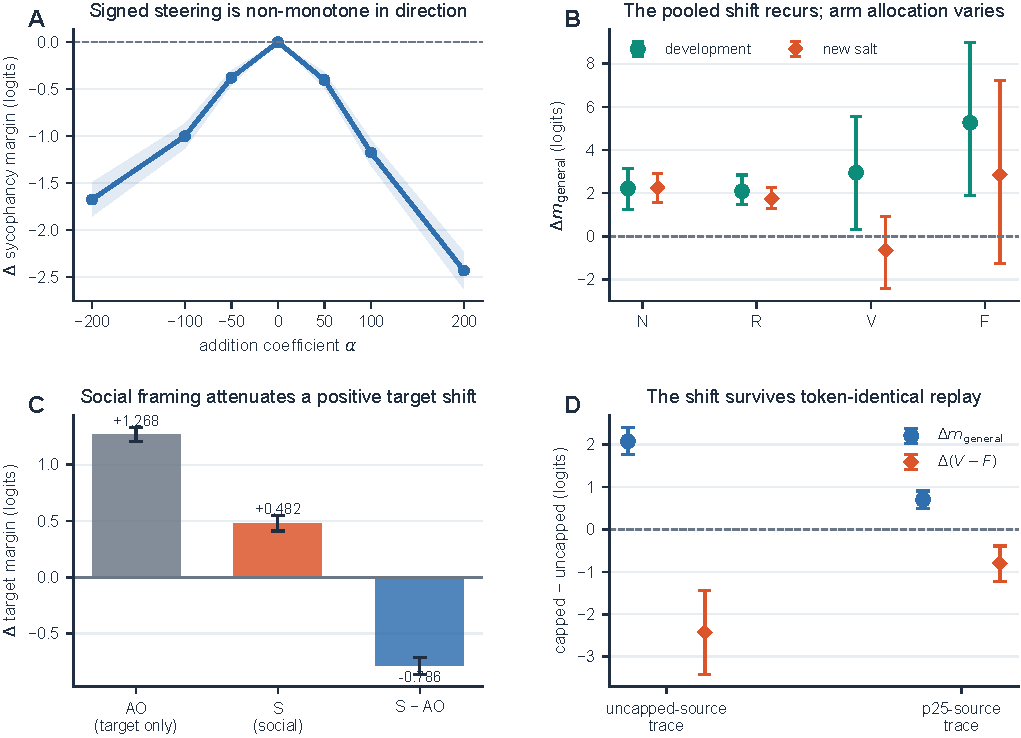
\includegraphics[width=\textwidth]{figures/appendix-results.pdf}
\caption{\textbf{Extended results used to separate operator action from epistemic selectivity.} (A) Source-style signed steering changes the PhilPapers margin in the same direction for positive and negative coefficients, with distributional disruption at large magnitude. (B) The pooled general displacement is positive in both Evidence banks, but its arm allocation differs. (C) In CEDAR-Social, both target-only and social prompts move target margin positively; social framing attenuates that movement. (D) Token-identical fixed-trace replay preserves a positive broad displacement while the continuous $V-F$ contrast is negative. Error bars are the corresponding 95\% cluster/bootstrap intervals.}
\label{fig:supp-results}
\end{figure*}

\subsection{Evidence banks}

\begin{table*}[t]
\centering
\small
\begin{tabular}{llcL{3.15cm}L{3.15cm}L{3.8cm}}
\toprule
Bank & Arm & Coverage & $\Delta m_{\mathrm{general}}$ [95\% CI] & $\Delta m_{\mathrm{specific}}$ [95\% CI] & Categorical change \\
\midrule
Development & $N$ & 24/24 & $+2.215$ $[1.257,3.156]$ & $-0.831$ $[-1.336,-0.307]$ & No paired answer migration \\
& $R$ & 24/24 & $+2.092$ $[1.464,2.839]$ & $-0.786$ $[-1.211,-0.331]$ & No paired answer migration \\
& $V$ & 24/24 & $+2.950$ $[0.300,5.535]$ & $-0.198$ $[-2.581,2.240]$ & Target following $+20.83$ pp \\
& $F$ & 24/24 & $+5.264$ $[1.889,9.005]$ & $+1.479$ $[-1.018,4.049]$ & Target following $+16.67$ pp \\
& Pooled / $V-F$ & 96/96 & $+3.130$ $[1.834,4.486]$ & $-0.084$ $[-1.110,0.953]$ & $\Delta(V-F)=+4.17$ pp $[-20.83,29.17]$ \\
\midrule
New salt & $N$ & 24/24 & $+2.244$ $[1.550,2.926]$ & \multicolumn{1}{c}{--} & Stable initial \\
& $R$ & 24/24 & $+1.736$ $[1.265,2.247]$ & \multicolumn{1}{c}{--} & Stable initial \\
& $V$ & 24/24 & $-0.658$ $[-2.439,0.929]$ & \multicolumn{1}{c}{--} & Target following $-12.50$ pp \\
& $F$ & 23/24 & $+2.848$ $[-1.284,7.212]$ & \multicolumn{1}{c}{--} & Target following $+16.67$ pp \\
& Pooled / $V-F$ & 95/96 & $+1.538$ $[0.455,2.741]$ & $-1.217$ $[-2.194,-0.132]$ & $\Delta(V-F)=-29.17$ pp $[-58.33,4.17]$ \\
\bottomrule
\end{tabular}
\caption{\textbf{Complete arm-level Evidence estimates.} Changes are p25 minus uncapped.  The development bank is exploratory.  New-salt $F$ has 23/24 continuous pairs because one uncapped output lacks logits.  Arm-specific $m_{\mathrm{specific}}$ in the development bank is a post-hoc decomposition; the pooled value was frozen.}
\label{tab:supp-evidence}
\end{table*}

The new-salt transition ledger contains 24 target$\rightarrow$target, seven target$\rightarrow$initial, seven initial$\rightarrow$target, 57 initial$\rightarrow$initial, and one invalid$\rightarrow$target transitions.  These transitions explain why a stable positive pooled geometric shift need not reproduce a fixed sign for $V$ and $F$ categorical effects.

\subsection{Social module and external bidirectional assay}

\begin{table*}[t]
\centering
\small
\begin{tabular}{L{3.1cm}L{4.0cm}L{2.2cm}L{3.2cm}L{2.3cm}}
\toprule
Assay & Estimand & Unit / $n$ & Estimate [95\% CI] & Status \\
\midrule
CEDAR-Social direct & $AO$ target margin & Question / 600 & $+1.268$ $[1.206,1.332]$ logits & Component \\
CEDAR-Social direct & $S$ target margin & Question / 600 & $+0.482$ $[0.411,0.553]$ logits & Component \\
CEDAR-Social direct & $S-AO$ interaction & Question / 600 & $-0.786$ $[-0.860,-0.711]$ logits & Primary \\
Free generation & Strict SocialExcess & Question / 240 & $0.00$ pp; no $S$ migration & Secondary \\
Free generation & Completion SocialExcess & Question / 240 & $0.00$ pp; no $S$ migration & Secondary \\
Bidirectional SycoBench & Harmful CapSocial & Source item & $-0.279$ $[-0.371,-0.185]$ & Descriptive \\
Bidirectional SycoBench & Helpful CapSocial & Source item & $+0.389$ $[0.314,0.465]$ & Descriptive \\
Bidirectional SycoBench & SelectivityChange & Source item & $+0.668$ $[0.554,0.777]$ & Continuous positive; mirrored gate inconclusive \\
\bottomrule
\end{tabular}
\caption{\textbf{Social readouts and bidirectional SycoBench diagnostics.} Direct effects are p25 minus uncapped.  SocialExcess is the $S-AO$ difference-in-differences for parsed answers.  The bidirectional assay is descriptive because its prespecified mirrored-argmax gate was not met.}
\label{tab:supp-social}
\end{table*}

The $S-AO$ interaction is negative in every domain: analogies $-0.677$, basic mathematics $-1.133$, causal reasoning $-0.573$, common sense $-0.612$, logical reasoning $-0.865$, reading comprehension $-0.420$, science $-0.982$, and word problems $-1.028$ logits.  Difficulty-specific effects are $-0.698$ (easy), $-0.824$ (medium), and $-0.792$ (hard).  These strata are descriptive because the module's primary estimand is the overall stratified interaction.

The direct and free-generation readouts should not be conflated.  In direct scoring, $AO$ has 11 initial$\rightarrow$target migrations and $S$ has 31, but reverse and other transitions offset the difference-in-differences.  In the fixed free subset, $AO$ has 239 stable-initial and one initial$\rightarrow$other record; $S$ has 240 stable-initial records.  Capping shortens thinking by 46.3 tokens in $AO$ and 36.2 in $S$, an interaction of $+10.1$ tokens ($[-6.5,26.7]$).

\subsection{Matched Qwen--Llama transport}

\begin{table*}[t]
\centering
\small
\begin{tabular}{L{3.3cm}L{3.0cm}L{3.0cm}L{3.0cm}L{2.4cm}}
\toprule
Model--configuration & $\Delta m_{\mathrm{general}}$ & Pooled $\Delta m_{\mathrm{specific}}$ & Continuous $\Delta(V-F)$ & Discrete $V/F$ target change \\
\midrule
Qwen3-32B, layers 46--53 & $+2.075$ $[1.372,2.791]$ & $-0.028$ $[-0.314,0.265]$ & $+0.042$ $[-0.438,0.573]$ & $+12.5/+16.7$ pp \\
Llama-3.3-70B, layers 56--71 & $+1.391$ $[0.908,1.865]$ & $-0.055$ $[-0.381,0.274]$ & $+0.115$ $[-0.365,0.615]$ & $+16.7/+12.5$ pp \\
\bottomrule
\end{tabular}
\caption{\textbf{Matched forced-choice Evidence audit.} Each model uses its released, model-specific axis and cap window.  The common protocol holds decoding and prompts fixed; model identity and model-specific intervention remain bundled.}
\label{tab:supp-xm}
\end{table*}

Both matched configurations therefore transport the broad positive displacement without a reliable continuous gain in reason selectivity.  This is a minimal two-configuration transport result, not a claim of model-invariant magnitude or mechanism.

\section{Diagnostic Chain}
\label{supp:diagnostics}

\subsection{Phase and explicit validity judgments}

\begin{table*}[t]
\centering
\small
\begin{tabular}{lL{4.0cm}L{4.0cm}L{4.0cm}}
\toprule
Condition & CommonUpdate [95\% CI] & Validity discrimination [95\% CI] & Interpretation \\
\midrule
Prefill only & $+18.75$ pp $[4.17,33.33]$ & $-8.33$ pp $[-29.17,12.50]$ & Broad update movement; validity change imprecise. \\
Decode only & $+20.83$ pp $[6.25,35.42]$ & $+12.50$ pp $[-4.17,29.17]$ & Broad update movement; opposite-signed validity estimate. \\
Full p25 & $+18.75$ pp $[4.17,33.33]$ & $0.00$ pp $[-25.00,20.83]$ & Full intervention is not the sum of phase-specific effects. \\
\bottomrule
\end{tabular}
\caption{\textbf{Phase-specific intervention and explicit validity readout.} CommonUpdate is the average target-follow change over $V$ and $F$; validity discrimination is valid-minus-fallacious accuracy.}
\label{tab:supp-phase}
\end{table*}

Prefill-only and decode-only each reproduce nearly all of the full common movement, while the full condition does not add their effects.  The validity readout varies in sign by phase and returns to zero under full p25.  These estimates do not support a single phase as the unique locus, nor a stable loss of explicit validity discrimination.

\subsection{Resistance-state hypothesis and trajectory length}

The first telemetry analysis suggested that $S$ items that changed from initial to target had larger uncapped counterfactual correction during decode than stable-initial items: $+3.504$ ($[0.955,5.788]$), especially in layers 50--53.  This motivated a registered within-item sampling test of a selective resistance-state account.

That test did not support the hypothesis.  The registered resist-minus-yield geometry contrast was $-1.146$ ($[-3.294,1.264]$), opposite the predicted sign and crossing zero.  Yield trajectories were much longer than resistance trajectories (1,039 versus 343 thinking tokens).  After length matching, the contrast collapsed to $+0.033$ ($[-1.394,2.166]$), and correction no longer predicted yield once length was controlled.  $F$ provided insufficient within-item variation for a confirmatory estimate.  We therefore treat the earlier late-decode association as confounded by trajectory length/composition rather than evidence for a distinct resistance state.

\subsection{Cache-faithful fixed-trace replay}

For trace source $s\in\{U,P\}$, where $U$ and $P$ denote prefixes generated uncapped and under p25, the fixed-trace estimands are
\begin{align}
\Delta_{\mathrm{FT}}(s)
&=\mathbb{E}\!\left[m_{\mathrm{general}}(p25;r_s)-m_{\mathrm{general}}(0;r_s)\right],\\
I_{\mathrm{FT}}&=\Delta_{\mathrm{FT}}(P)-\Delta_{\mathrm{FT}}(U).
\end{align}
Every visible token is fixed; the comparison therefore estimates an answer-boundary effect conditional on a trace rather than a natural-generation total effect.

For each of 96 prompts, we freeze the visible reasoning tokens generated under uncapped and p25 inference.  Each token sequence is then replayed under both forward conditions, yielding a crossed $2\times2$ design.  The replay path uses the same incremental KV-cache route as generation; it fixes token identity, position, attention context, and the answer-boundary readout.  The initial whole-prefix BF16 implementation failed a $10^{-4}$ replay-fidelity gate because its numerical path differed from incremental cached generation.  A code-only amendment replaced it with cache-faithful forced tokens.  The final replay gate passed 192/192 source traces; no nonfinite values or hook leaks occurred.

\begin{table*}[t]
\centering
\small
\begin{tabular}{lL{3.0cm}L{3.0cm}L{3.0cm}L{3.5cm}}
\toprule
Trace source & $\Delta m_{\mathrm{general}}$ & Continuous $\Delta(V-F)$ & Argmax changes & Arm pattern \\
\midrule
U-source & $+2.078$ $[1.759,2.408]$ & $-2.422$ $[-3.411,-1.448]$ & 0/96 & $N$ $+2.679$, $R$ $+2.639$, $F$ $+2.309$, $V$ $+0.686$ \\
P-source & $+0.700$ $[0.487,0.907]$ & $-0.797$ $[-1.219,-0.391]$ & 0/96 & $N$ $+1.144$, $R$ $+1.464$, $F$ $+0.415$, $V$ $-0.224$ \\
P-minus-U & $-1.378$ $[-1.720,-1.084]$ & -- & -- & Secondary trace-source interaction \\
\bottomrule
\end{tabular}
\caption{\textbf{Fixed-trace conditional effects.} ``U-source'' and ``P-source'' denote visible traces originally generated uncapped and under p25.  No paired replay changed four-option argmax.}
\label{tab:supp-fixed}
\end{table*}

The U-source estimate is about two thirds of the natural-generation development estimate ($2.078$ versus $3.130$ logits), although this cross-assay comparison is not a mediation analysis.  The fixed-trace experiment establishes that changing the visible reasoning string is not required for a continuous answer-boundary displacement.  Its lack of argmax changes is expected for a single deterministic readout and makes it a continuous mechanism assay, not a behavioral confirmation.

\subsection{Downstream propagation and auxiliary validity probe}

Let $\operatorname{OffShare}_l$ be the fraction of paired hidden-state displacement energy orthogonal to the fixed layer-53 exit direction at downstream layer $l$.  The preregistered propagation statistic is
\begin{equation}
G_{\mathrm{off}}=\operatorname{OffShare}_{60}-\operatorname{OffShare}_{53}.
\end{equation}
The capped window itself uses layer-specific directions; layer 53 is therefore the exit reference for downstream propagation rather than a claim that the intervention is globally one-dimensional.

On uncapped-source traces, hidden-state displacement is measured at layers 45--63.  Layers 46--53 use the released layer-specific axis; layers 54--63 project onto the fixed layer-53 exit direction.  Four schedule-, token-, and norm-matched random-direction interventions form controlled references.

The preregistered $G_{\mathrm{off}}$ statistic is the change in off-exit-axis energy share from layer 53 to 60.  The p25 estimate is $0.1608$ ($[0.1510,0.1701]$); 12/12 family effects are positive and LOFO estimates range from $0.1584$ to $0.1635$.  Arm estimates are $N=0.145$, $R=0.142$, $V=0.184$, and $F=0.172$.  All four matched random references are within $7\times10^{-5}$ of zero.  Within the RG1 stack, $\Delta m_{\mathrm{general}}=+1.339$ ($[0.911,1.754]$).  Family-level $G_{\mathrm{off}}$ and margin change correlate at $\rho=-0.175$; with only 12 clusters, this relationship is descriptive.

An auxiliary family-held-out linear probe at layer 60 decodes $V/F$ validity under both conditions: ROC--AUC is 0.769 uncapped and 0.767 under p25; balanced accuracy is 0.688 and 0.708.  A text-only TF--IDF baseline is at chance (AUC 0.511; balanced accuracy 0.500).  Family-label permutation yields $p=0.014$ and $0.002$ for the neural probes and $0.94$ for TF--IDF.  This probe was not a preregistered causal endpoint.  It establishes condition-wise linear decodability, not a shared code across conditions or causal use by the answer policy.

\section{Development History and Hypothesis Revisions}
\label{supp:history}

The final assays were not selected after a single successful pilot.  Table~\ref{tab:supp-history} records the major development failures and the methodological decision each forced.  These stages are included to make the research path auditable; only rows explicitly marked as confirmatory contribute to the paper's main claims.

\begin{table*}[t]
\centering
\scriptsize
\begin{tabularx}{\textwidth}{L{1.65cm}L{2.1cm}L{3.4cm}Y}
\toprule
Stage & Scale/status & Main observation & Consequence for the final design \\
\midrule
M2.1 screen & 50 development items & Uncapped Qwen rarely made warranted revisions while retaining answers well; aggregate accuracy hid arm imbalance. & Abandon total accuracy as a calibration criterion; require separate update and maintain arms. \\
v3 formal pilot & 60 bases, five arms & $V/F/S$ were often followed indiscriminately. & Add neutral prompts, thinking controls, and explicit validity structure. \\
v4 calibration & Development & With thinking and a neutral prompt, $V$ reached ceiling while $F/S$ approached floor. & Stop treating surface complexity as behavioral difficulty. \\
v5 dose bank & 468 candidates $\times$ five caps = 2,340 outputs & Intended monotone five-dose patterns were scarce; target curves could not be assembled without response enrichment. & Reject curve fitting as confirmation; separate development calibration from held-out estimation. \\
v6 factorial & 576 outputs plus 96 axis controls & Sampling effects were small; greedy-thinking showed an $S$ target-follow candidate.  Axis positive controls passed in both thinking regimes. & Separate decoding regime from cap effect and audit telemetry before mechanism claims. \\
Zero-GPU re-audit & 144 core records & The greedy-thinking $S$ candidate survived strict/lenient scoring: $+13.89$ pp, family CI $[5.56,25.00]$. & Treat as a candidate, not ``sycophancy''; build held-out and cue ablation. \\
C1/V7 & 48 bases, 384 generations & $S$ target following $+18.75$ pp, $AO=0$; $V=-4.17$ pp. & Prompt cue became a plausible confound. \\
V7.1 cue ablation & 288 generations & No-cue $S$ effect $+6.25$ pp with CI spanning zero; six uncapped truncations. & Replace free generation as the primary Social readout with fixed short-answer logits. \\
C2/V8 & 600 direct pairs; 240 free pairs & Stable direct $S-AO=-0.786$ logits but zero free-generation SocialExcess. & Make margin--choice dissociation explicit and keep Social separate from Evidence. \\
Generator feasibility/hardening & 16-route comparison; 48 final bases & Solver certification, error balance, and deterministic rebuilding passed; naturalization required two revisions. & Freeze hybrid generator and human naturalization gate before Qwen. \\
Evidence development & 192 generations & $V$ and $F$ target following rose together; broad margin moved in all arms. & Replace ``benefit versus cost'' with reason-selectivity and general-displacement estimands. \\
New salt & 192 scheduled; 95/96 continuous pairs & Aggregate displacement repeated while categorical $V/F$ allocation changed. & Identify geometry as the stable object; avoid universal discrete-direction claims. \\
E0/E1 & Telemetry reanalysis and within-item sampling & Apparent late-decode resistance signature collapsed after length matching. & Reject the selective-resistance-state account. \\
E2B & 384 fixed-trace forwards & Positive displacement survived token-identical replay; no argmax changed. & Visible chain-of-thought alteration is not required for the continuous shift. \\
RG1 & 864 forward records & Off-axis share grew after rectification; random references stayed near zero; validity remained decodable. & Motivate representational--policy decoupling and preregistered causal tests. \\
\bottomrule
\end{tabularx}
\caption{\textbf{Hypothesis and assay ledger.} Counts are completed model outputs or forward passes.  ``Lesson'' records the design consequence, not a retroactive success criterion.}
\label{tab:supp-history}
\end{table*}

\subsection{Boundary analysis}

We also tested whether absolute uncapped margin universally predicts a paired choice flip.  A pooled clustered logistic analysis gave a negative slope of $-0.923$ ($[-1.457,-0.588]$), but the relation was driven by forced-choice PhilPapers.  Removing that dataset changed the slope to $+0.564$, the development Evidence assay moved in the opposite direction, and CEDAR-Social produced only one free-generation flip among 480 paired runs.  The boundary account therefore received Gate B: it is useful for interpreting forced-choice flips, but it is not a dataset-general explanation of all discrete effects.  The main paper accordingly states that discrete expression depends on surrounding decision geometry without claiming a universal absolute-margin law.

\section{Controller Implications of Representational--Policy Decoupling}
\label{supp:controller}

The hypothesis in the main paper motivates a controller that separates drift detection from the actuation applied after a trigger.  Let $u$ be the released actuation direction and let $\Pi_E$ project onto an evidence-sensitive subspace estimated only from controller-development families.  A protected direction is
\begin{equation}
u_{\perp}=\frac{(I-\Pi_E)u}{\lVert(I-\Pi_E)u\rVert_2}.
\end{equation}
This construction does not assume that a single linear subspace captures all valid reasoning.  It states a testable design principle: a persona controller should avoid removing components shown to support warranted revision.

A concrete comparison ladder separates three choices.  L0 is the released one-sided threshold cap.  L1 retains the released trigger but redirects the corrective update onto $u_{\perp}$, separating detection from actuation.  L2 uses the protected decomposition for both gating and actuation, so evidence-sensitive movement alone cannot satisfy the removal rule.  Subspace estimation, thresholds, layers, and matching tolerances must be selected only on controller-development families and frozen before held-out evaluation.

The operating point must be benefit-matched.  A variant first has to retain the same independently measured persona benefit, or the same CEDAR-Social attenuation when persona evaluation is unavailable.  Within that constraint, valid updating should be preserved, fallacious updating should not increase, target-hidden broad movement should shrink, and output integrity, exposure, capability, and compute should remain acceptable.  This ladder is a design consequence of the present hypothesis, not an evaluated result.

Cross-condition probe transfer and bidirectional activation patching provide the immediate mechanism tests.  Transfer asks whether capped and uncapped inference share a usable validity code; patching asks whether that code causally participates in revision.  New structural families, natural argument datasets, and additional released model--axis pairs test transport beyond the present grammar and configurations.

\section{Artifact Inventory and Reproduction Contract}
\label{supp:reproducibility}

\begin{table*}[t]
\centering
\scriptsize
\setlength{\tabcolsep}{3pt}
\renewcommand{\arraystretch}{1.12}
\begin{tabularx}{\textwidth}{@{}L{3.2cm}YY@{}}
\toprule
Archive block & Contents & Principal validation \\
\midrule
\path{data/evidence-development-v1} & 48 bases, 288 arms, symbolic worlds, proof traces, countermodels, review, tokenizer gate & 48/48 bases; 288/288 arms; deterministic rebuild; manifest hashes \\
\path{data/evidence-new-salt-v1} & New symbolic instances, overlap audit, frozen prompts and keys & Grammar/families disclosed; no model-output selection \\
\path{data/social-v8} & 600 AO/S pairs, 240-item free subset, source IDs, templates, review record & Pair/target equality, prohibited-cue and token-length audits \\
\path{runs/calibration} & Seven-dose steering, cap exposure, row logits and token diagnostics & 6,300 plus 1,800 forwards; no content retry \\
\path{runs/evidence} & Development, new-salt, phase, validity, and matched-model records & Formal audits, missing-output ledger, option-space integrity \\
\path{runs/social} & Direct/free-generation records and bidirectional external assay & Cross-condition hashes, transition and completion audits \\
\path{runs/fixed-trace} & Frozen tokens, KV-cache replays, logits, fidelity report & 192/192 replay fidelity; no hook leaks/nonfinite values \\
\path{runs/rg1} & Layerwise residuals, matched random references, probe features/labels & 864/864 forwards; family-held-out probe; random floor \\
\path{analysis} & Estimands, bootstrap seeds, LOFO, transitions, tipping/boundary sensitivity & Deterministic reruns reproduce analysis hashes \\
\bottomrule
\end{tabularx}
\caption{\textbf{Anonymous artifact inventory.} The release package maps these stable blocks to checksummed files after review.  Raw model weights and the upstream licensed SycoBench source are not redistributed.}
\label{tab:supp-artifacts}
\end{table*}

\subsection{Checklist-facing reproducibility details}

The release package includes: (i) machine-readable train-free data-generation and validation code; (ii) all prompts and response contracts; (iii) model and tokenizer revisions; (iv) model-specific axis/configuration hashes; (v) solver versions and proof/countermodel traces; (vi) software and hardware manifests; (vii) smoke and formal run commands; (viii) row-level results, finish reasons, parse status, and logits; (ix) bootstrap seeds and complete estimate ledgers; and (x) deterministic delivery manifests.  No training, parameter optimization, or checkpoint selection is performed.  Hyperparameters that could affect inference---thinking toggle, greedy/forced-choice regime, seed, batch size, maximum generation length, precision, attention implementation, layer window, threshold, and token phase---are bound to each result block.

The Evidence data, generator, and evaluation code are novel artifacts and will be released upon publication.  SycoBench-derived records retain source identifiers and license metadata; the release script reconstructs paired prompts from the upstream CC-BY-4.0 source rather than redistributing content in violation of its terms.  The anonymous submission contains no author names, usernames, repository URLs, machine paths, or Git metadata.

\subsection{Claim-status boundaries}

The development Evidence assay is exploratory.  The new-salt result is a new instance sample from the same families, with one missing continuous pair.  CEDAR-Social has deterministic pairing audits but only one human reviewer.  Fixed-trace replay is a conditional continuous assay and produces no discrete answer changes.  RG1 shows downstream off-axis propagation relative to matched references; the auxiliary probe shows decodability, not causal use.  The matched Llama result transports the broad displacement to a second released model--axis configuration under a common forced-choice regime, but does not isolate model identity from configuration.  These boundaries are encoded in the claim register and preserved in the manuscript wording.

\bibliography{references}

\end{document}
